\chapter{Query Overview, Results and Evaluation}\label{results}
To analyse the functionality of the database systems, I devised a number of queries with ranging difficulties. The aim of the queries was to establish the limitations of the systems, and to discover the efficacy of the systems. A further objective was to identify any extra features the solutions provide which may be useful. For example any visualisations of graphical analysis which may enhance the exploration of the data. Chapter \ref{evaluationstrategy} provides a detailed explanation of the reasoning behind the queries. This chapter discusses the output and results of running the queries in the various query languages. This chapter also gives insight into the difficulty of writing the query, the usefulness of the output, the time taken for the query to run and any challenges I faced when throughout the process. Additionally included in this chapter is a general discussion which summarises the capabilities of the systems and aims to provide one with an understanding of the limitations of each of the systems (section  \ref{queryevaluation}).

\section{Query Overview}\label{output}
The screen captures, tables, graphs and charts illustrated in this chapter are based on the results of running the competency based queries on each database system. Table \ref{tab:competency} details each of the devised queries in English, provides a short description of the data expected to be returned and includes a rating characterisation. The rating characterisation ranges from 1 to 5, and while there is no science behind the rating it is to be used as a guide to aid the reader into understanding \textbf{1.} General complexity of the query. \textbf{2.} Fruitfulness of the data returned. \textbf{3.} Level of expectancy that the system will be able to accomplish the query (on a scale of 1 expected, to 5 unexpected).

The order in which I wrote, run and evaluated the queries reflects the complexity of the query itself. I started by implementing simple queries which one would expect each of the systems to successfully achieve. The difficulty of each query increased every time. The end point of this evaluation was when I had written a number of complex queries which would be used to assess the EMAGE dataset in real life scenarios. For example, query number 7 in table \ref{tab:competency} ``Calculate transitive closure''. Finding the hierarchical path of a structure is something which researchers and scientists are often trying to achieve when analysing an anatomy. For example in terms of a human anatomy, the finger is part of the hand which is joined to the wrist which is part of the arm which is joined to the shoulder and so forth. Therefore its inclusion in this examination was necessary. A full description of this query, its origins and output is provided below. 

\begin{table}[H]
\centering
\resizebox{\textwidth}{!}{
\begin{tabular}{|c|l|l|c|}
\hline
\textbf{Query Number} & \multicolumn{1}{c|}{\textbf{English}} & \multicolumn{1}{c|}{\textbf{Expected return}} & \textbf{Rating} \\ \hline
1 & All structures at Theiler Stage X. & Theiler Stage and Structure ID. & 1 \\ \hline
2 & \begin{tabular}[c]{@{}l@{}}All structures between Theiler\\ Stage X and Y.\end{tabular} & \begin{tabular}[c]{@{}l@{}}Structure ID, Theiler Stage X and Theiler Stage\\Y.\end{tabular} & 1 \\ \hline
3 & Where is Gene X expressed? & \begin{tabular}[c]{@{}l@{}}Name of the gene, the structure where the\\ gene was found and the EMAGE ID where the\\ gene was found.\end{tabular} & 2 \\ \hline
4 & What is expressed in structure X? & \begin{tabular}[c]{@{}l@{}}Name of the gene(s) found in the structure. The\\structure ID and the name of the structure.\\ The Theiler Stage(s) of the structure. The\\EMAGE ID of the structure.\end{tabular} & 3 \\ \hline
5 & \begin{tabular}[c]{@{}l@{}}Which genes are stored in\\ structures X and Y?\end{tabular} & \begin{tabular}[c]{@{}l@{}}Name and ID of the gene(s). The ID of\\structure X and ID of structure Y.\end{tabular} & 4 \\ \hline
6 & \begin{tabular}[c]{@{}l@{}}Which Genes are most\\ commonly co-expressed?\end{tabular} & \begin{tabular}[c]{@{}l@{}}Name of the gene(s) and the count of unique\\ structures the gene is expressed in.\end{tabular} & 5 \\ \hline
7 & Calculate transitive closure. & The name of each structure and its parent. & 5 \\ \hline
\end{tabular}}
\caption{Competency queries for each database system.}
\label{tab:competency}
\end{table}

There are a number of queries one could write which would output potentially interesting results and provide an alternative view of the data. However, the purpose of this examination was to evaluate the functionality of the solutions, assess the limitations of each of the systems and identify any interesting additional features. Thus there was no requirement to include these additional queries which would fail to affect the outcome of the examination.

\section{Query Results}\label{queryresults}
The following subsections provide the results of running the queries outlined in table \ref{tab:competency}. Included in the subsections is the statement written for every system for each of the queries, where I was able to achieve the intended outcome. I have also included the physical output for the first query for each database. This is to provide the reader with an insight into what is returned from each database solution when running a query. I have only included the output for the first query as I felt that doing the same process for each query did not add any value to the examination.

\subsection*{Query 1 - All structures at Theiler Stage X}\label{query1}
The first query which I wrote for each of the databases aimed to retrieve the anatomy structure information at a given Theiler Stage. For the basis of these tests I hard coded the Theiler stage; Theiler Stage 4 in this instance.  The minimum amount of data expected to be returned from this query is the structure ID, structure name and Theiler Stage. This query is not complex and one would expect that each database will possess the required functionality to handle this query and return the expected output.

\subsubsection*{MySQL - Query 1 statement}\label{mysqlquery1statement}
The MySQL query shown in code snippet \ref{code:mysqlquery1} successfully returned the expected output. The query was straightforward and only required a single join of the Stages and Anatomy Structures table. I was able to use the ``AS'' keyword to manually define an alias for the column headings of the returned data. The use of this keyword enhances the clarity of the output and allows one to easily identify the data being represented, as illustrated in figure \ref{fig:mysqlquery1}. Without the inclusion of the ``AS'' keyword, the headings of the returned data would be the same as the column names in the select statement. For example, ``StructureID'' would be ``AnatomyStructures.accession'' and ``StructureName'' would be ``AnatomyStructures.term''. The official MySQL documentation suggests It is good practice to explicitly use the ``AS'' keyword for all column names \cite{mysqlworkbench}.

\begin{lstlisting}[language=SQL, caption=MySQL Query 1 statement. All structures at Theiler Stage 4, label=code:mysqlquery1]
SELECT t1.accession AS StructureID, t1.term AS StructureName, t2.theilerstage AS TheilerStage, t2.dpc AS DPC
FROM AnatomyStructures AS t1
INNER JOIN Stages AS t2
ON t1.stage_id = t2.id
WHERE t2.theilerstage = 4
ORDER BY 1
\end{lstlisting}

\subsubsection*{MySQL - Query 1 output}\label{mysqlquery1output}
Figure \ref{fig:mysqlquery1} is a screen capture of the resulting output from running the MySQL query in the command-line interface. As you can see it returns the data in a table format separated by dashed lines. The number of rows returned and time taken for the query to process is also included below the table.

The output for this query is clear and coherent. However, for this query there is only 4 columns of data being returned. The MySQL command-line tool is run in a machine terminal. The size of the terminal window is at maximum the size of the machines monitor. Thus it is often the case that when returning a large number of columns, the data can become scrambled and illegible.

\begin{figure}[H]\begin{center}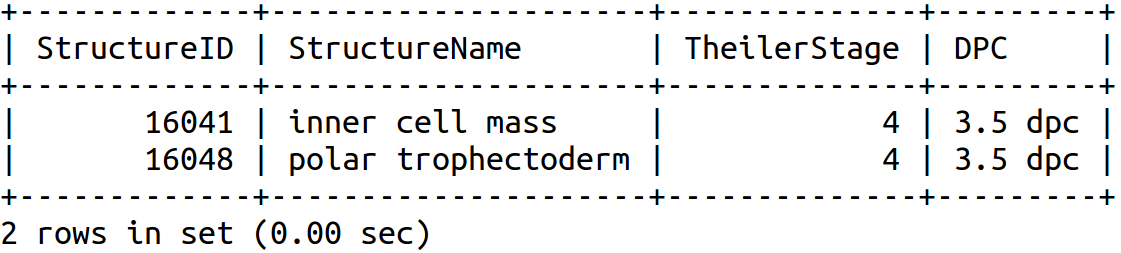
\includegraphics[height=4cm,width=0.9\linewidth]{images/mysqlquery1}\caption{Screen capture MySQL command-line tool output - Query 1}\label{fig:mysqlquery1}\end{center}\end{figure}

One way to avoid this is to change the zoom level of the terminal. Depending on the volume of data returned, this can have little to no affect as the further out one zooms, the smaller the font becomes. This can often be a hindrance of using the MySQL command-line tool for advanced queering of large, multicolumn datasets.

\subsubsection*{MongoDB - Query 1 statement}\label{mongoquery1statement}
The MongoDB query shown in code snippet \ref{code:mongoquery1} successfully returned the expected output. To retrieve the data I used the \textit{db.collection.find()} command. The query is made up of two main parts. Firstly the query matches the field and value in the curly brackets. This is shown in line 2 of code snippet \ref{code:mongoquery1}. This line alone would have successfully returned the required data. However, it would have also returned the rest of data in the document, such as the publication and specimen information. As I was only looking to pull the Theiler Stage, structure term and structure ID, I had to include an additional parameter to the query.

The second part of this query is known as the projection. Within the projection, one can specify fields to exclude from the result. Lines 5-9 in code snippet \ref{code:mongoquery1} represent the projection of this query. A field can be included or excluded from a result by specifying the relevant field and then stating either 1 (included) or 0 (excluded) value. Doing so, allows one to filter the result and only return the fields required.
\begin{lstlisting}[language=json, caption=MongoDB Query 1 statement. All structures at Theiler Stage 4., label=code:mongoquery1]
db.emage.find(
	{	"stage.theilerstage":4	},
    {	"_id" : 0,
    "stage.theilerstage" : 1,
    "stage.dpc" : 1,
    "textannotation.anatomystructure.structureID" : 1,
    "textannotation.anatomystructure.term" : 1	}	).pretty();
\end{lstlisting}

One additional command which concludes this query is the ``pretty()'' method. This command displays the results in an easy-to-read format. A standard \textit{db.collection.find()} query outputs data in a dense and incomprehensible format. Using the ``pretty()'' method returns the data in a format which is easier for humans to understand.

\subsubsection*{MongoDB - Query 1 output}\label{mongoquery1output}
Figure \ref{mongoquery1output} illustrates the results returned from running query 1 in MongoDB. The query was run on the MongoDB command-line tool. As with MySQL, when running a query which may return a large volume of data, the command-line interface can often be difficult to view the results. However, with the inclusion of the ``pretty()'' method, analysing the field and value pairs of a MongoDB document is greatly enhanced.
\begin{figure}[H]\begin{center}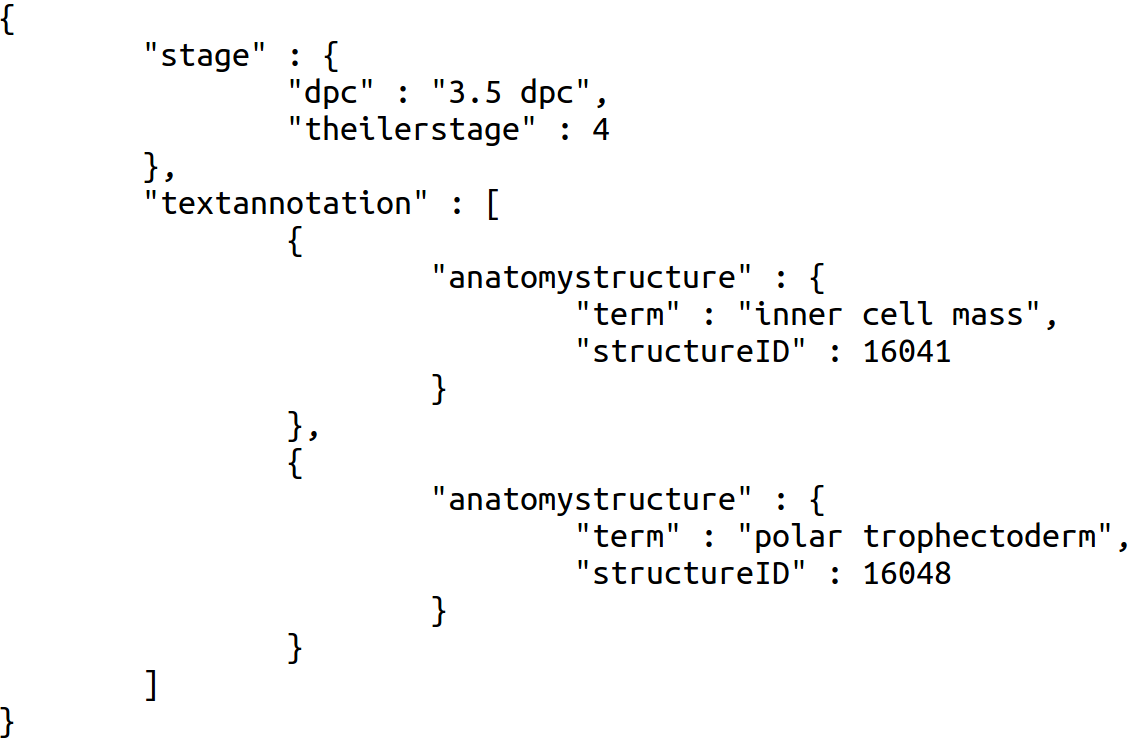
\includegraphics[width=1\linewidth]{images/mongoquery1}\caption{MongoDB command-line tool output - Query 1}\label{fig:mongoquery1}\end{center}\end{figure}

\subsubsection*{Neo4j - Query 1 statement}\label{neoquery1statement}
The Neo4j query shown in code snippet \ref{code:neoquery1} successfully returned the expected output. Cypher, the Neo4j query language, while uniquely different, is similar to SQL. They both share many of the same functions and methods. One distinctive difference is that Cypher queries specify the data to be returned at the end of the query, as opposed to the start. Despite this dissimilarity, the structure and format of SQL and Cypher queries are very similar.

Line 1 in code snippet \ref{code:neoquery1} is indicative of this. The ``MATCH'' command, firstly begins the query, and also specifies which nodes the data will be pulled from. This is the equivalent of a SQL ``FROM'' keyword. For example, ``(struct:AnatomyStructure)'' specifies the data will come from an ``AnatomyStructre'' node and for the basis of the query the alias will be ``struct''. This is the same for the ``Stage'' node. Also included in line 1 is the relationship which will join the ``AnatomyStructure'' and ``Stage'' nodes. One can either explicitly state the relationship between the nodes, in the square brackets. Alternatively, using an empty set of brackets or stating just an alias, will tell the system to find the relationship between the nodes regardless of its value.
\begin{lstlisting}[language=SQL, caption=Neo4j Query 1 statement. All structures at Theiler Stage 4, label=code:neoquery1]
MATCH (struct:AnatomyStructure)-[Relationship]->(stage:Stage)
WHERE stage.theilerStage = 4
RETURN struct.structureID AS StructureID, Relationship, stage.theilerStage AS TheilerStage, stage.dpc AS DPC;
\end{lstlisting}
\parindent 0pt
For example, in this query, the relationship between the nodes is ``GROUPED\_BY''. However, as I have just provided an alias, the system will match whichever relationship it finds between the nodes.

\parindent 15pt
Line 2 of code snippet \ref{code:neoquery1} is a standard ``WHERE'' clause. It has the same semantic value as an SQL ``WHERE'' clause. Finally the query is finished with a ``RETURN statement'', found on line 3. This is equivalent to a SQL ``SELECT'' command. One specifies the field and value pairings as required. As with MySQL it is good practice to use alias names, and can be done so by expressing the ``AS'' keyword.

\subsubsection*{Neo4j - Query 1 output}\label{neoquery1output}
By default Neo4j provides two tools for querying the database and outputting the result. The first is on the Neo4j command-line tool; a basic command-line interface for querying a database. The way it works is similar to that of MySQL, MongoDB and Cassandra; start the tool, connect to a database, then run a query.

\begin{figure}[H]\begin{center}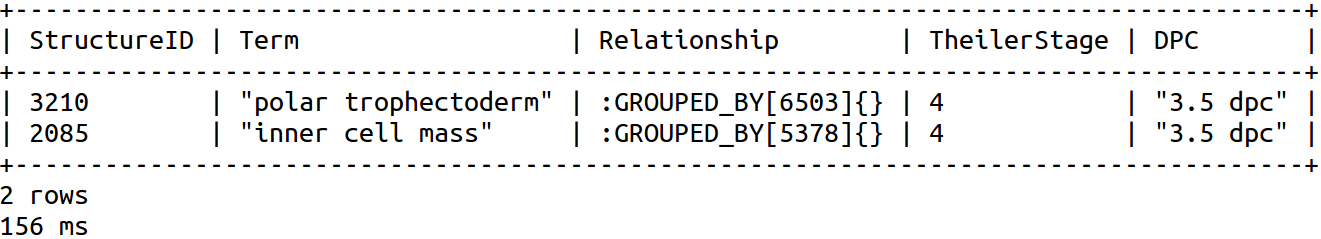
\includegraphics[height=4cm,width=0.9\linewidth]{images/neo4jquery1terminal}\caption{Neo4j query 1 - All structures at Theiler Stage X}\label{fig:neo4jquery1terminal}\end{center}\end{figure}

The output from running the query in code snippet \ref{code:neoquery1} using the command-line tool is illustrated in figure \ref{fig:neo4jquery1terminal}. The output is almost identical with that of MySQL. This does not come as a surprise as Neo4j is based on SQL constructs. It is a basic format however it meets the needs for most.

A reason why the creators of Neo4j did not differ from the norm regarding the command-line interface, may be down to the fact they have developed a web interface for querying Neo4j models. The web browser application comes as standard with the community edition (the most basic version) of Neo4j. It is the primary user interface for Neo4j. Using this application one can run queries in the same manner as running queries on the command-line tool. The application also displays the nodes, relationships and constraints of the data mode. It is designed to provide one with a intuitive, user-friendly experience of Neo4j.

\begin{figure}[H]\begin{center}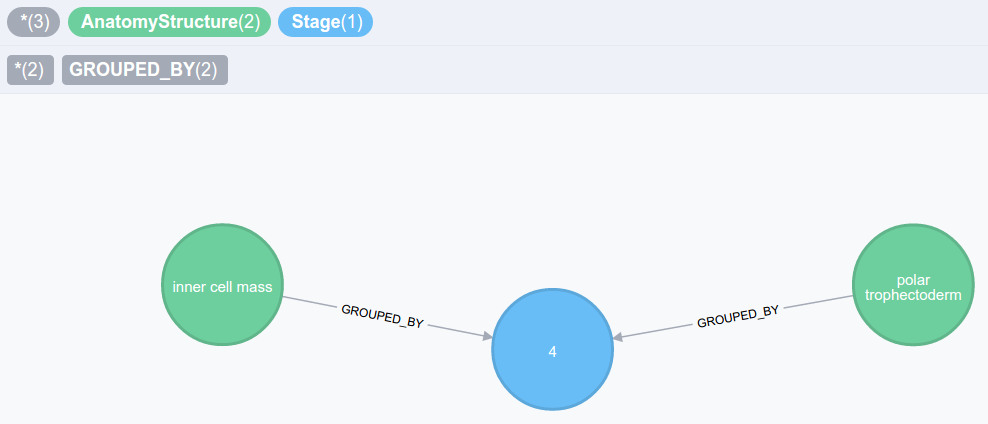
\includegraphics[width=1\linewidth]{images/neo4jquery1graph}\caption{Neo4j query 1 - All structures at Theiler Stage X}\label{fig:neo4jquery1graph}\end{center}\end{figure}

One feature of the application is its graph visualisation tool. Illustrated in figure \ref{fig:neo4jquery1graph}, the web interface allows one to view the result of their query as a graph. The nodes and relationships displayed, represents the of the query in code snippet \ref{code:neoquery1}. The colours, sizes and labels of the nodes are fully customisable and one can move (by dragging) the nodes around the screen at ones convenience.

The visualisation tool is basic, but easy to use. Its inclusion in the application enhances the usability of Neo4j, for those who are looking for an alternative way of viewing their data. However, it is not very robust. While running a query which returns a large volume of data may not take a long time to run, representing the data in the interface can take some time to load. Furthermore, the web interface is also prone to crashing when returning a lot of data.

It is often the case when querying a database using an API or otherwise, that one intends on loading the data into a visualisation tool or implementing a solution to model the data. Therefore rendering the addition of this application obsolete. That said, it is a useful tool for basic data visualisation and database querying.

\subsubsection*{Apache Cassandra - Query 1 statement}\label{cassquery1statement}
Code snippet \ref{code:cassquery1} represents the query written to find all of the structures found at a given Theiler Stage in the Cassandra data model. The Cassandra query language uses similar syntax to that of MySQL. They both share many of the same keywords and the structure of a query is the same. Start with selecting the columns you need for the query, state which table the data is stored in and then include any clauses to match the data on.

The query is much shorter and simpler compared with the MySQL statement for the same query. This is as a result of the inability for Cassandra to join tables. Therefore all of the data required to output the result of this query is stored in the one table.

\begin{lstlisting}[language=SQL, caption=, label=code:cassquery1]
SELECT *
FROM structurebystage
WHERE theilerstage = 4
AND detected = true;
\end{lstlisting}

\subsubsection*{Apache Cassandra - Query 1 output}\label{cassquery1output}
The output of running the query in code snippet \ref{code:cassquery1} can be found in figure \ref{fig:cassandraquery1}. As with Neo4j, to the naked eye, the output of running queries on the command-line looks very similar to that of MySQL. Despite how Cassandra is semantically structured, visually, there is not much dissimilarity.

One difference with Cassandra is the colouring of the column headings. The colours themselves have no significance on how the table is structured, and are dependent on the configuration of ones terminal window. However, the positioning and distinctness of the colours, do have a bearing on the table structure. In the instance of figure \ref{fig:cassandraquery1}, the initial two columns coloured red represent the partitioning keys, defined in section \ref{cassandraimplementation}. The cyan coloured column represents the clustering key, and the pink coloured headings define the remaining columns. In terms of the data, the green coloured values depict either an Integer or a Boolean value and the purple coloured data represents a String.

\begin{figure}[H]\begin{center}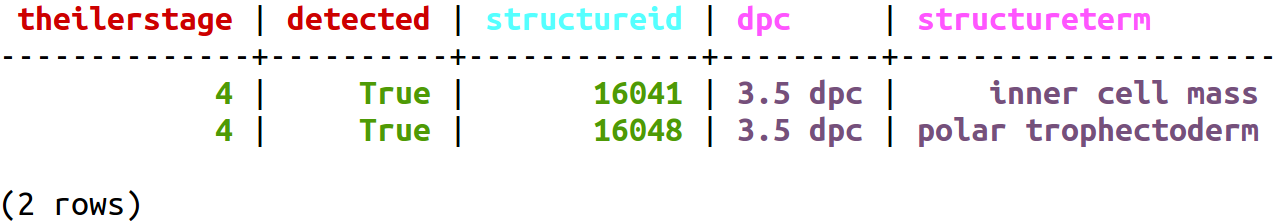
\includegraphics[height=4cm,width=0.9\linewidth]{images/cassandraquery1}\caption{Cassandra query 1 - All structures at Theiler Stage X}\label{fig:cassandraquery1}\end{center}\end{figure}

In terms of the effectiveness of this feature, it certainly makes the output easier on the eye and more attractive from a aesthetic standpoint. However, I feel it adds little to the overall impact of the data returned. Depending on the role of the user querying the database, having a colour coordinated keys and data types may have little impact. For example, if one is designing the data model in a Database Administrator type role, colours representing the partitioning and clustering keys can be useful. It allows one to see exactly how the table is structured without having to run a further query to describe the table. Having coloured data values also shows whether a number is indeed an Integer or a String for example. Comparatively, if one is in a business type role and does not understand the underlying architecture of the database, then the various colours may confuse or complicate their analysis. While having many colours does give the output an interesting look and feel, it does not improve the querying experience. It does seem that this feature is to primarily enhance the practicality of the database when querying, which it only achieves to an extent.

\subsection*{Query 2 - All structures between Theiler Stage X and Y}\label{query2}
The second query aimed to identify all of the structures found between two given Theiler Stages. For each of the queries I used the same minimum and maximum Theiler Stages values (4 and 7). This is a query which one would anticipate each of the systems would complete with relative ease. The data expected to be returned from the query is, as a minimum, the structure ID and the corresponding Theiler Stage. 

\subsubsection*{MySQL - Query 2 statement}\label{mysqlquery2statement}
The MySQL query shown in code snippet \ref{code:mysqlquery2} successfully returned the expected output. To construct the query I had to write two inner joins. The first linking the AnatomyStructures table to the Stages table, and the second joining the AnatomyStructures table to the TextAnnotation table.

\begin{lstlisting}[language=SQL, caption=, label=code:mysqlquery2]
SELECT t1.accession, t2.theilerstage
FROM AnatomyStructures AS t1
INNER JOIN Stages AS t2
ON t1.stage_id = t2.id
INNER JOIN TextAnnotations AS t3
ON t1.id = t3.structure_id
WHERE t2.theilerstage BETWEEN 4 AND 7
AND t3.detected = 1
GROUP BY 1;
\end{lstlisting}

I have imposed two clauses on the query, found in lines 7 and 8 of code snippet \ref{code:mysqlquery2}. The first, on lune 7 stipulates the Theiler Stage must have a value between 4 and 7. On line 8 I specify that the gene must have a boolean value of 1; detected. The GROUP BY clause on line 9, is used to group the result-set by column 1 (structure ID). This will return a distinct set of structure ID values.

The query was straightforward to create. Compared to Neo4j and Cassandra however, it was a long query in terms of syntax. This can often be the case when writing relational database queries. The more tables in the data model, the longer and more complex the query becomes.

\subsubsection*{MongoDB - Query 2 statement}\label{mongoquery2statement}
The MongoDB query shown in code snippet \ref{code:mongoquery2} successfully returned the expected output.

\parindent 0pt
\begin{lstlisting}[language=json, caption=, label=code:mongoquery2]
db.emage.find(
	{ $and:
		[
			{	"textannotation.detected" : "True"	},
			{	"stage.theilerstage": {$gte : 4 }	},
			{	 "stage.theilerstage": {$lte : 7 }	},
			{	"textannotation.strength" : "detected"	}
		]
	},
	{	"textannotation.anatomystructure.structureID" : 1, "stage.theilerstage" : 1, "_id" : 0	}	).pretty();
\end{lstlisting}

MongoDB supports a number of logical and comparison query operators. These include \$and (logical and), \$gte (>=) and \$lte (<=), each of which are used in the query below.

\parindent 15pt

The \$and logical operator denotes field and value pairs must all satisfy the arguments provided, for a query to return true, within an array of two or more expressions. It is semantically the same as a logical AND. If one of the arguments returns false, MongoDB will not evaluate the remainder of the expression. The \$gte and \$lte operators select the documents where the value of the field is either greater/less than or equal to a specified value.

\subsubsection*{Neo4j - Query 2 statement}\label{neoquery2statement}
The Neo4j query shown in code snippet \ref{code:neoquery2} successfully returned the expected output. This was a basic query and I found it easy to construct as it was extremely similar to that of the MySQL query created previously.

\begin{lstlisting}[language=SQL, caption=, label=code:neoquery2]
MATCH (textannotation:TextAnnotation)-[]->(struct:AnatomyStructure)-[]->(stage:Stage)
WHERE stage.theilerStage >= 4 AND stage.theilerStage <=7 AND textannotation.detected = 1
RETURN struct.accession AS Accession, stage.theilerStage AS TheilerStage;
\end{lstlisting}

\subsubsection*{Apache Cassandra - Query 2 statement}\label{cassquery2statement}
The Cassandra query shown in code snippet \ref{code:cassquery2} successfully returned the expected output. This was a simple query and quick to write. This was mainly due to the fact I had modelled the table around such an query.

\begin{lstlisting}[language=SQL, caption=, label=code:cassquery2]
SELECT *
FROM structurebystage
WHERE theilerstage IN (4,5,6,7)
AND detected = true;
\end{lstlisting}

One noteworthy point from this query is the use of the IN operator. Cassandra Query Language only supports the use of = and IN operators when restricting a partition key within a query. Therefore as opposed to using either >= or the BETWEEN operators in MySQL, MongoDB and Neo4j, for Cassandra I had to hard-code the physical values I was restricting the column on. This is illustrated in line 3 of code snippet \ref{code:cassquery2}.

\subsection*{Query 3 - Where is gene X expressed?}\label{query3}
The third query I created was to test if the systems could successfully return information regarding a given gene. This query is slightly more complex as it requires more clauses within the queries. However, one would again expect that each of the solutions should be able to return the expected data with ease. I chose the gene ``Hoxb13'' as the gene to test the queries. For the solution to be deemed successful in running this query I would expect the gene name, structure name and structure ID to be returned, as a minimum.

\subsubsection*{MySQL - Query 3 statement}\label{mysqlquery3statement}
The MySQL query shown in code snippet \ref{code:mysqlquery3} successfully returned the expected output. 

\begin{lstlisting}[language=SQL, caption=, label=code:mysqlquery3]
SELECT t1.name AS GeneName, t3.term AS StructureTerm, t3.accession AS StructureID
FROM Genes AS t1
INNER JOIN TextAnnotations AS t2
ON t1.id = t2.gene_id
INNER JOIN AnatomyStructures AS t3
ON t2.structure_id = t3.id
WHERE t2.detected = 1
AND t1.name = 'Hoxb13'
GROUP BY 3
ORDER BY 2,3;
\end{lstlisting}

\subsubsection*{MongoDB - Query 3 statement}\label{mongoquery3statement}

\begin{lstlisting}[language=json, caption=, label=code:mongoquery3]
db.emage.find(
	{	$and:
		[
			{	"textannotation.gene.name": "Hoxb13"	},
				{	$or:
					[
						{	"textannotation.strength": "detected"	},
						{	"textannotation.strength": "strong"	}
					]
				}
	}	).pretty();
\end{lstlisting}

\subsubsection*{Neo4j - Query 3 statement}\label{neoquery3statement}

\begin{lstlisting}[language=SQL, caption=, label=code:neoquery3]
MATCH (g:Gene)<-[]-(textannotation:TextAnnotation)-[]->(a:AnatomyStructure)
WHERE g.name = 'Hoxb13' AND textannotation.detected = 1
RETURN g.name AS Name, a.accession AS  StructureID, a.term AS Term
ORDER BY a.accession ASC
\end{lstlisting}

\subsubsection*{Apache Cassandra - Query 3 statement}\label{cassquery3statement}

\begin{lstlisting}[language=SQL, caption=, label=code:cassquery3]
SELECT *
FROM structurebygene3
WHERE genename = 'Hoxb13'
AND detected = true
ALLOW FILTERING;
\end{lstlisting}

\subsection*{Query 4 - What is expressed in structure X?}\label{query4}
This query was designed to identify the data which is expressed in a given structure. With the inclusion of this query, the complexity has again increased however, one would expect each of the solutions to successfully achieve this query. The data returned from this query is what makes it interesting. The ability to view what information is contained within a given structure, provides an essential analytical insight into the data. The minimum data expected to be returned from this query is the gene name, structure ID, structure term, Theiler Stage and EMAGE ID.

\subsubsection*{MySQL - Query 4 statement}\label{mysqlquery4statement}

\begin{lstlisting}[language=SQL, caption=, label=code:mysqlquery4]
SELECT t1.name AS GeneName, t2.accession AS StructureID, t2.term AS TermName, t4.theilerstage AS TheilerStage, t3.emage_id AS EMAGE_ID
FROM Genes AS t1
INNER JOIN emage.TextAnnotations AS t3
ON t1.id = t3.gene_id
INNER JOIN emage.AnatomyStructures AS t2
ON t3.structure_id = t2.id
INNER JOIN Stages AS t4
ON t2.stage_id = t4.id
INNER JOIN Assays AS t5
ON t3.emage_id = t5.emage_id
WHERE t3.detected = 1
AND t2.accession = 17451
ORDER BY 5;
\end{lstlisting}

\subsubsection*{MongoDB - Query 4 statement}\label{mongoquery4statement}

\begin{lstlisting}[language=json, caption=, label=code:mongoquery4]
db.emage.find(
	{	"textannotation.anatomystructure.structureID": 17451	},
	{	},
	{	"_id":1}	).pretty();
\end{lstlisting}

\subsubsection*{Neo4j - Query 4 statement}\label{neoquery4statement}

\begin{lstlisting}[language=SQL, caption=, label=code:neoquery4]
MATCH (stage:Stage)<-[]-(struct:AnatomyStructure)<-[]-(text1:TextAnnotation)-[]->(assay:Assay)
WHERE struct.accession = 17451
RETURN struct.accession AS StructureID, struct.term AS Term,stage.theilerStage AS TheilerStage, assay.emageID AS EMAGEID
ORDER BY assay.emageID ASC
\end{lstlisting}

\subsubsection*{Apache Cassandra - Query 4 statement}\label{cassquery4statement}

\begin{lstlisting}[language=SQL, caption=, label=code:cassquery4]
SELECT *
FROM textannotations1
WHERE structureid = 17451
AND detected = true
ALLOW FILTERING;
\end{lstlisting}

\subsection*{Query 5 - Which Genes are stored in structures X and Y?}\label{query5}
The following code snippets represent the queries written for competency question 5.

\subsubsection*{MySQL - Query 5 statement}\label{mysqlquery5statement}

\begin{lstlisting}[language=SQL, caption=, label=code:mysqlquery5]
SELECT t1.name AS GeneName
FROM Genes AS t1
INNER JOIN TextAnnotations AS t3
ON t1.id = t3.gene_id
INNER JOIN AnatomyStructures AS t2
ON t2.id = t3.structure_id
WHERE t3.detected = 1
AND t2.accession IN (16062, 16069)
GROUP BY 1
HAVING COUNT(DISTINCT t2.accession) > 1;
\end{lstlisting}

\subsubsection*{Neo4j - Query 5 statement}\label{neoquery5statement}

\begin{lstlisting}[language=SQL, caption=, label=code:neoquery5]
MATCH (n:Gene)<-[]-(t:TextAnnotation)-[]->(a:AnatomyStructure)
with count (distinct (a.accession)) as c, t as ta, a as an, n as ge
WHERE ta.detected = 1 and an.accession = 16062 or an.accession = 16069 and c > 1
return distinct ge.name
order by ge.name
\end{lstlisting}

\subsection*{Query 6 - Which Genes are most commonly co-expressed?}\label{query6}
The following code snippets represent the queries written for competency question 6.

\subsubsection*{MySQL - Query 6 statement}\label{mysqlquery6statement}


\begin{lstlisting}[language=SQL, caption=, label=code:mysqlquery6]
SELECT t1.name AS GeneName, COUNT(DISTINCT t2.accession) AS Co_Expressed_Count
FROM Genes AS t1
INNER JOIN TextAnnotations AS t3
ON t1.id = t3.gene_id
INNER JOIN AnatomyStructures AS t2
ON t2.id = t3.structure_id
WHERE t3.detected = 1
GROUP BY 1
HAVING COUNT(DISTINCT t2.accession) > 1
ORDER BY 2 DESC
LIMIT 5;
\end{lstlisting}

\subsection*{Query 7 - Calculate transitive closure}\label{query7}
The following code snippets represent the queries written for competency question 7.

\subsubsection*{MySQL - Query 7 statement}\label{mysqlquery7statement}

\begin{lstlisting}[language=SQL, caption=, label=code:mysqlquery71]
SELECT DISTINCT tmp.term, t1.parent_term AS lev1, t2.parent_term AS lev2, t3.parent_term AS lev3, t4.parent_term AS lev4
FROM Closure AS t1
INNER JOIN AnatomyStructures AS tmp
ON t1.child_id = tmp.accession
LEFT JOIN Closure AS t2 ON t2.child_id = t1.parent_id
LEFT JOIN Closure AS t3 ON t3.child_id = t2.parent_id
LEFT JOIN Closure AS t4 ON t4.child_id = t3.parent_id
WHERE tmp.accession = 16201
\end{lstlisting}

\begin{lstlisting}[language=SQL, caption=, label=code:mysqlquery72]
SELECT distinct tmp.term, t1.parent_term AS lev1, t2.parent_term as lev2, t3.parent_term as lev3, t4.parent_term as lev4, t5.parent_term as lev5, t6.parent_term as lev6
FROM Closure AS t1
INNER JOIN AnatomyStructures as tmp
ON t1.child_id = tmp.accession
LEFT JOIN Closure AS t2 ON t2.child_id = t1.parent_id
LEFT JOIN Closure AS t3 ON t3.child_id = t2.parent_id
LEFT JOIN Closure AS t4 ON t4.child_id = t3.parent_id
LEFT JOIN Closure AS t5 ON t5.child_id = t4.parent_id
LEFT JOIN Closure AS t6 ON t6.child_id = t5.parent_id
WHERE tmp.accession = 16205;
\end{lstlisting}